%chktex-file 44
\subsection{Introduction}
Characteristics according to ISO 9126: FURP ME
\begin{itemize*}
\item \textbf{Functionality}\\
 suitability accuracy, security, compliance, interoperability
\item \textbf{Usability}\\
 understandability, learnability, operability
\item \textbf{Reliability}\\
 maturity, fault tolerance, recoverability
\item \textbf{Portability}\\
 Adaptability, intallability, conformance, replaceability
\item \textbf{Maintainability}\\
 Analysability, changeability, stability, testability
\item \textbf{Efficiency}\\
 time behaviour, resource utilization
\end{itemize*}

\textbf{Testing and quality:}\\
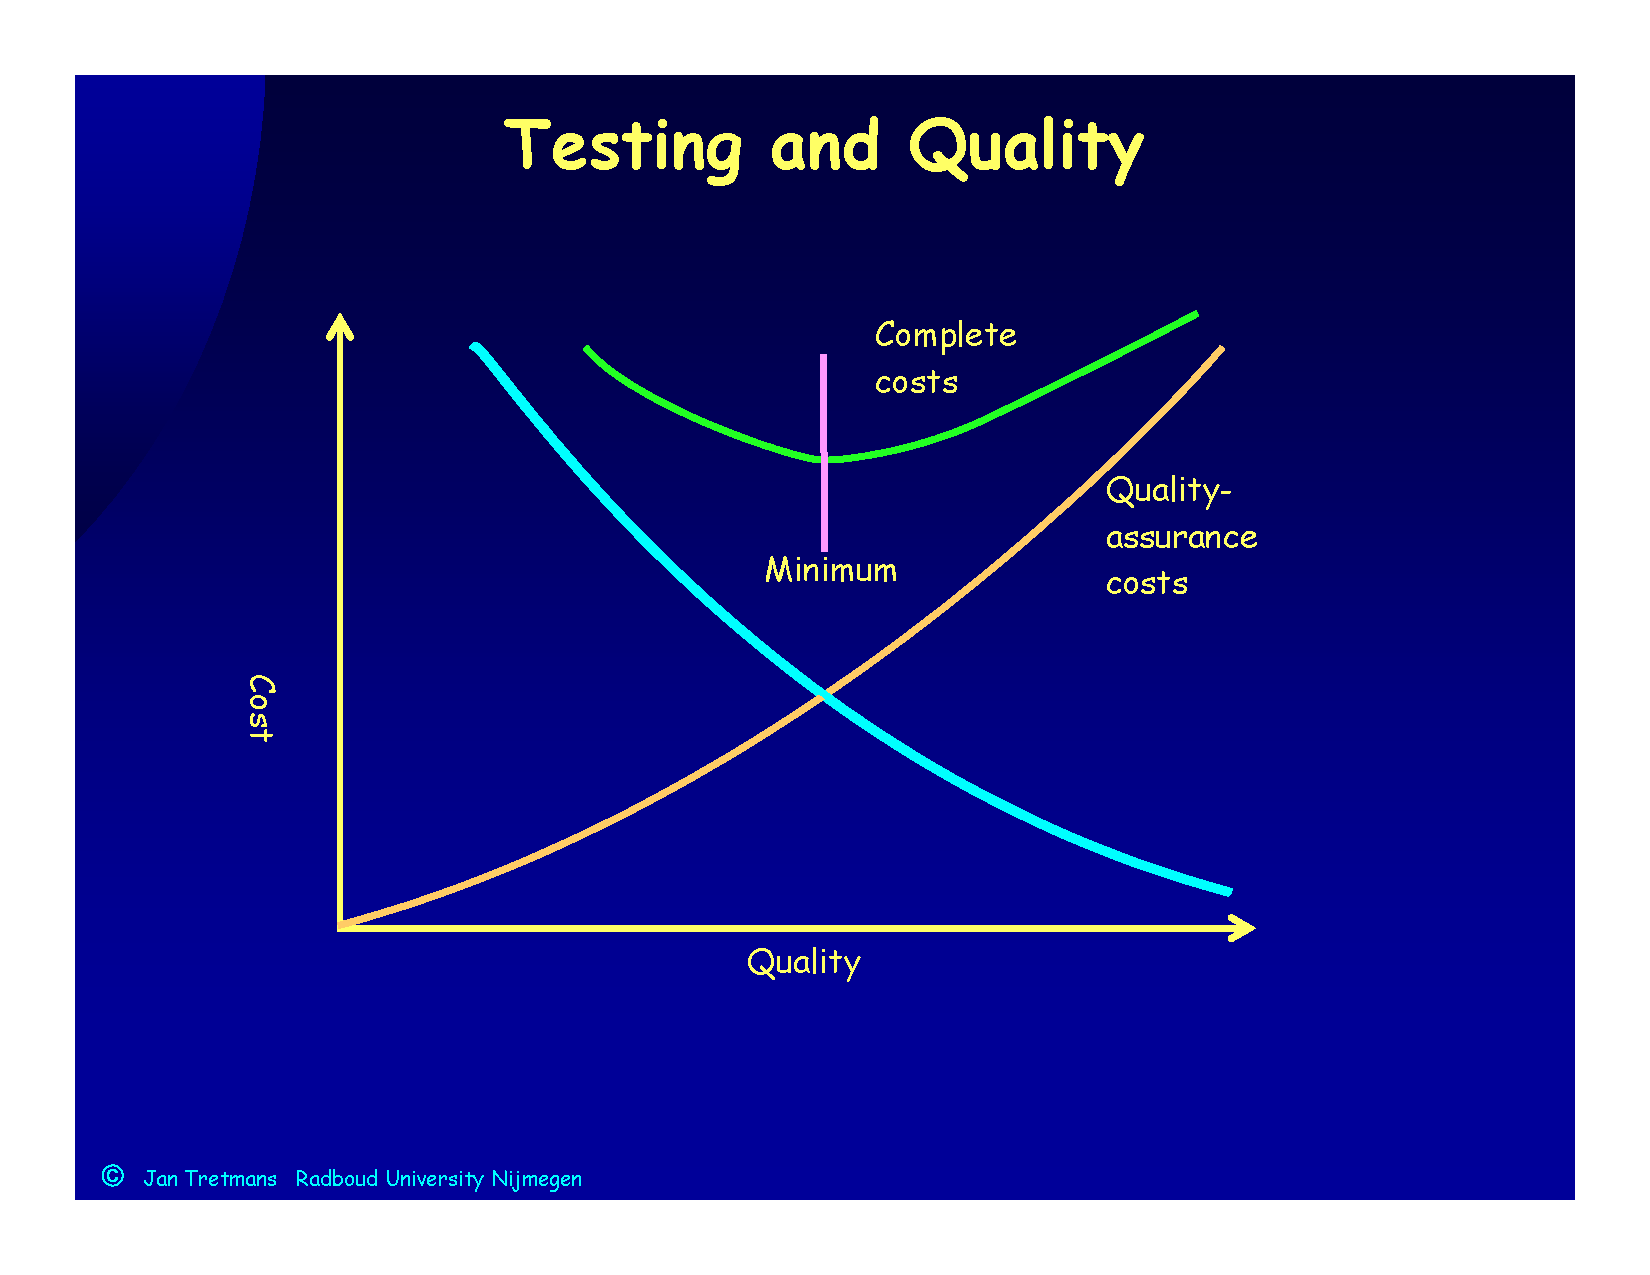
\includegraphics[width=0.8\linewidth,clip,trim=4cm 4cm 6cm 5cm]{testingQC.pdf}

\begin{tabularx}{\linewidth}{r|X}
	Failure  & observed incorrect behaviour of the IUT, result of a fault \\ 
	\hline Fault  & problem in the program causing the failure \\ 
    \hline Defect & detected failure (by tester)\\ 
	\hline Issue & politically correct term for failure. Used when you do not know whether the test is wrong or the system is wrong \\ 
	\hline Error & can only be made by a human being  \\ 
	\hline Bug & fault \\ 	
\end{tabularx} 

\subsubsection{sorts of testing}

\textbf{Quality characteristics:}
\begin{multicols}{2}
\begin{itemize*}
	\item functional
	\item error
	\item security
	\item compliance
	\item interoperability
	\item reliability
	\item robustness
	\item usability
	\item learnability
	\item performance
	\item resource
	\item stress
	\item portability
	\item conformance
\end{itemize*}
\end{multicols}

\textbf{Who:}
\begin{itemize*}
	\item developer
	\item tester
	\item acceptance
	\item user
	\item certification
	\item production
\end{itemize*}

\textbf{Phase:}
\begin{itemize*}
	\item unit
	\item integration
	\item module
	\item system
	\item regression
	\item duration
\end{itemize*}

\textbf{Black box}
\begin{itemize*}
	\item no internal details of software considered
	\item based on externally observable behaviour
\end{itemize*}

\textbf{White box}
\begin{itemize*}
	\item based on structure of the code
	\item “oracle” required
\end{itemize*}

\textbf{Grey box}
\begin{itemize*}
	\item anything between black and white
	\item e.g.\ component based testing
\end{itemize*}

\subsubsection{Verification \& Validation}
\begin{itemize*}
	\item Verification = building the product right
	\begin{itemize*}
		\item concerns development process
		\item intermediate products
		\item e.g.\ checking the testability of the specification
	\end{itemize*}
	\item Validation = building the right product
	\begin{itemize*}
		\item whether final product meets requirements and needs
		\item e.g.\ by reviewing the specification
	\end{itemize*}
\end{itemize*}




